\chapter{Introduction} 

\section{Solver theory}

\subsubsection{Euler}
Take derivative, multiply with timestep, add to initial value, repeat until end.

\subsubsection{Runge-Kutta methods}
Take derivatives at some time points, multiply with proper coefficients, add all to intial value, repeat until end.

\section{Functional programming}
Don't know whether I should add a section on this in order to make everything understandable for people not familiar with FP/Haskell.

\section{Solving ordinary differential equations in Haskell}
\lstset{style=haskellStyle}

Functional languages have several properties which make them suitable for the purpose of solving problems in numerical mathematics.
\begin{itemize}
	\item Haskell notation close to mathematics + partial function application + referential transparency
	\item Clear type system for (1) checking errors/eliminating wrong implementations and (2) quick glance at what the program does
	\item Declarative -- hide the details and let the exact execution be figured out by the compiler. You simply specify what you want as answer.
	\item Reasonably high performance \cite{Bench}
\end{itemize}

\lstinputlisting[firstline=18]{../haskell/SolverTypes.hs}
The types in Haskell reveal lots of information about the structure and functionality of the program. The three main types making up the numerical solver for ordinary differential equations are listed above.

\begin{figure}[h!]
	\caption{A picture of a gull.}
	\centering
	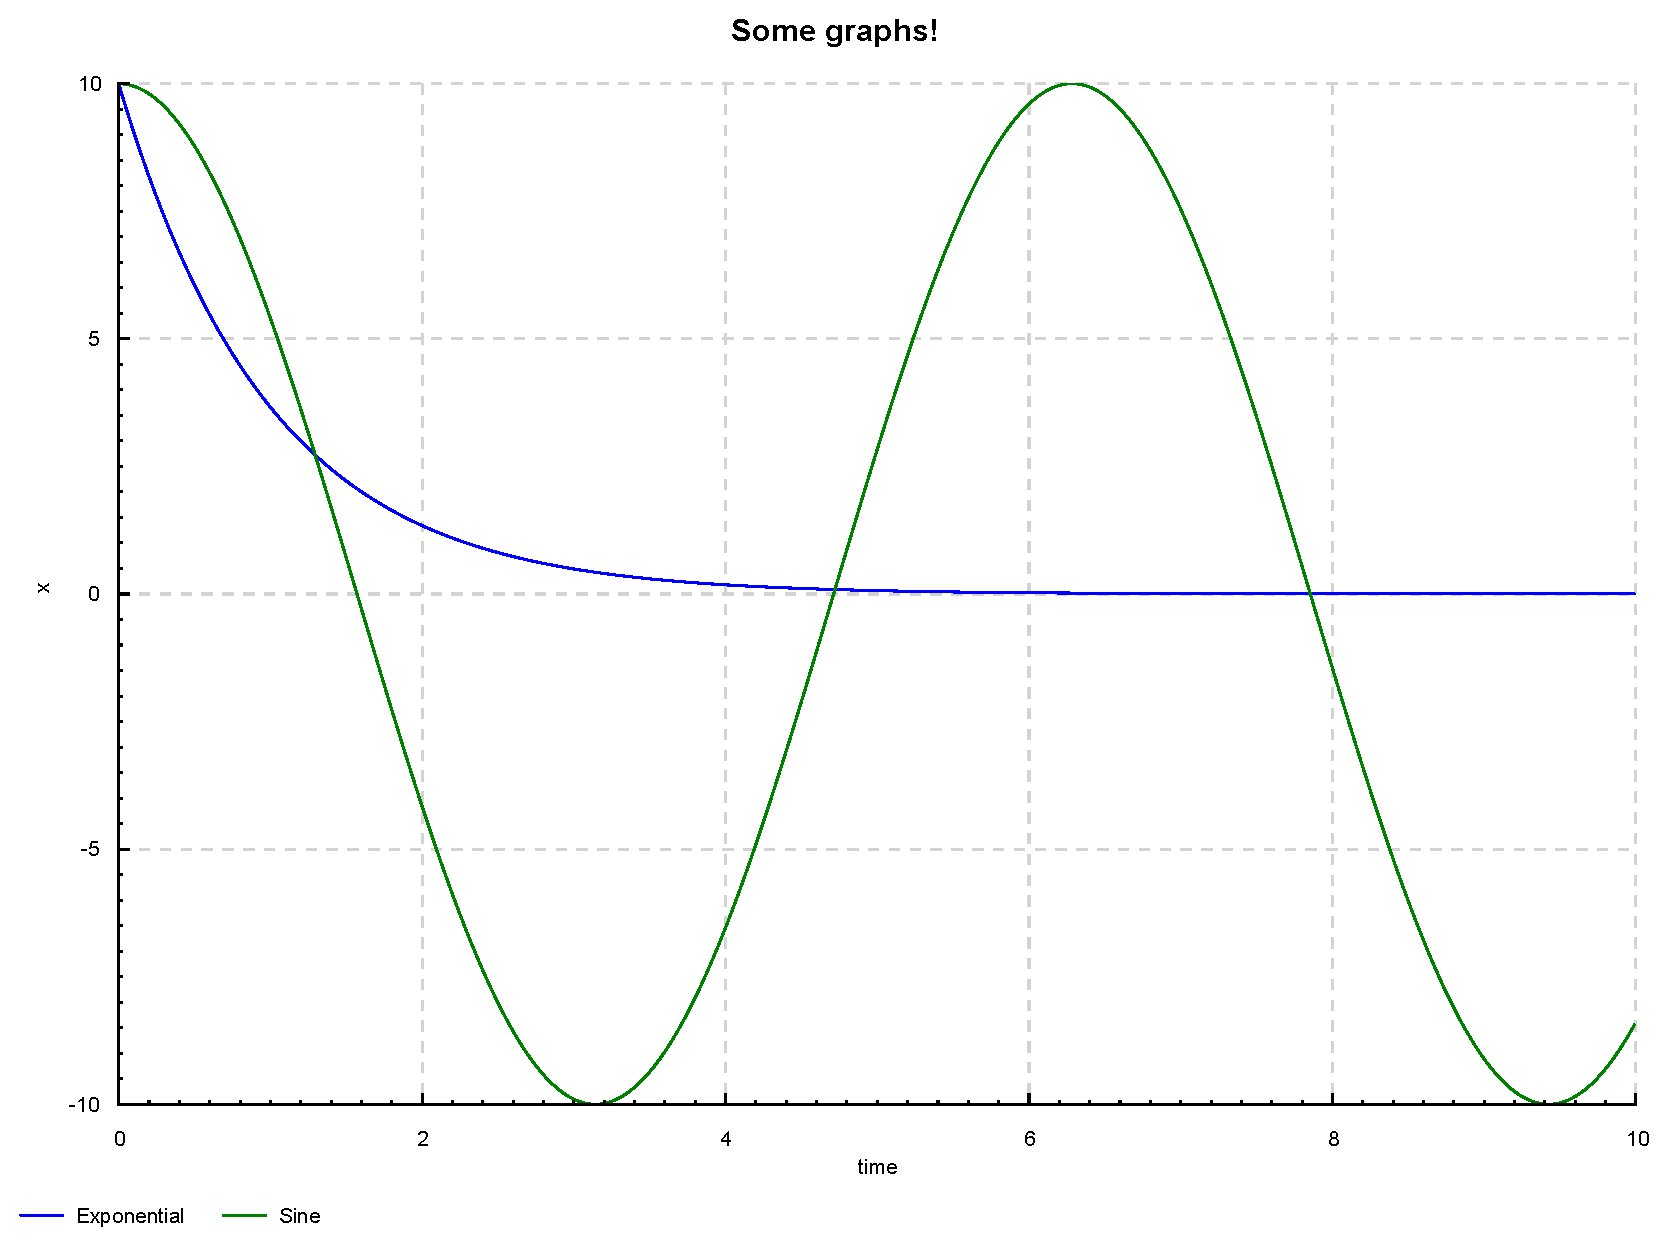
\includegraphics[width=0.5\textwidth]{../haskell/output.pdf}
\end{figure}

\section{Conversion to Mealy Machines}

\section{FPGAs}
\begin{itemize}
	\item What are FPGAs used for?
	\item Why should I care about FPGAs
	\item What is the current workflow for programming FPGAs
\end{itemize}


\section{Data transfer to \LaTeX{} ?}


The most famous equation in the world: $E^2 = (m_0c^2)^2 + (pc)^2$, which is 
known as the \textbf{energy-mass-momentum} relation as an in-line equation.

A {\em \LaTeX{} class file}\index{\LaTeX{} class file@LaTeX class file} is a file, which holds style information for a particular \LaTeX{}.

Lorem Ipsum is simply dummy text of the printing and typesetting industry. Lorem Ipsum has been the industry's 
standard dummy text ever since the 1500s, when an unknown printer took a galley 
of type and scrambled it to make a type specimen book. It has survived not only 
five centuries, but also the leap into electronic typesetting, remaining 
essentially unchanged. It was popularised in the 1960s with the release of 
Letraset sheets containing Lorem Ipsum passages, and more recently with desktop 
publishing software like Aldus PageMaker including versions of Lorem 
Ipsum.